\documentclass[conference,onecolumn,a4paper]{IEEEtran}

\usepackage[utf8]{inputenc}
\usepackage[T1]{fontenc}
\usepackage[hidelinks]{hyperref}
\usepackage{graphicx}
\usepackage{url}
\usepackage{hyphenat}
\usepackage{float}
\usepackage{fancyvrb}
\usepackage{wrapfig}
\usepackage{subcaption}

\begin{document}

\title{
    \Huge{User Manual} \\
    \large{Information Security Project}
}

\author{
    \IEEEauthorblockN{\small{Daniel Planötscher, 19615 \texttt{dplanoetscher@unibz.it}}}
    \IEEEauthorblockN{\small{Leo Kerschbaumer, 19072, \texttt{lekerschbaumer@unibz.it}}}
    \IEEEauthorblockN{\small{Roland Bernard, 19598 \texttt{rolbernard@unibz.it}}}
}

\maketitle
\thispagestyle{plain}
\pagestyle{plain}

\section{Getting Started}

\subsection{Requirements}

\begin{itemize}
    \item Maven\footnote{\url{https://maven.apache.org/}}
    \item Java 17 JDK\footnote{\url{https://www.oracle.com/java/technologies/downloads/\#java17}}
\end{itemize}

The application is written in Java using features introduced with Java version 17. For compiling the project, it is therefore required to install the Java JDK version 17 or later. The Maven software is used for dependency management and must be installed on the system for the recommended install procedure.

\subsection{Installation}

To quickly download the source for this application, compile it, and start the secure version of the project execute the following commands.

\begin{verbatim}
git clone https://github.com/rolandbernard/is-project
cd ./is-project/secure/
mvn compile spring-boot:run
\end{verbatim}

Installation and compilation from source is handled thought Maven. After cloning the git repository of this project, you will three different projects located within it. The insecure version of the application can be found in the directory \verb|insecure/|, while the secure version is located in \verb|secure|. The third project inside the repository at \verb|rainbow/| contains an implementation of rainbow tables and tools for generating and using them.

\subsection{Starting}

To compile one of the projects, navigate into the proper directory (e.g., \verb|cd ./is-project/secure/|) and execute the Maven command \verb|mvn compile|. Maven will automatically download all required dependencies and compile the classes in the project. Then, to start the server of either the secure or insecure web application execute the Maven command \verb|mvn spring-boot:run|. The project is using the Spring Boot\footnote{\url{https://spring.io/projects/spring-boot}} framework for handing web interaction. Additionally, we use a Maven plugin that allows starting the web server using this simple command.

After starting the web server, the application will be available on port 8080. You can navigate to \verb|http://localhost:8080| in your browser to access it. Note that the secure version of the application will redirect you to the HTTPS version of the site at \verb|https://localhost:8443|. Since the default certificate contained in the repository is self-signed, most browsers will give you a warning saying that the site is not secure. In order to use the applicaion with the distributed certificate, you should tell the browser to accept the risk and continue to \verb|https://localhost:8443|. This option is often hidden behind the “Advanced” button.

\begin{figure}[H]
    \centering
    \begin{subfigure}[b]{0.4\linewidth}
        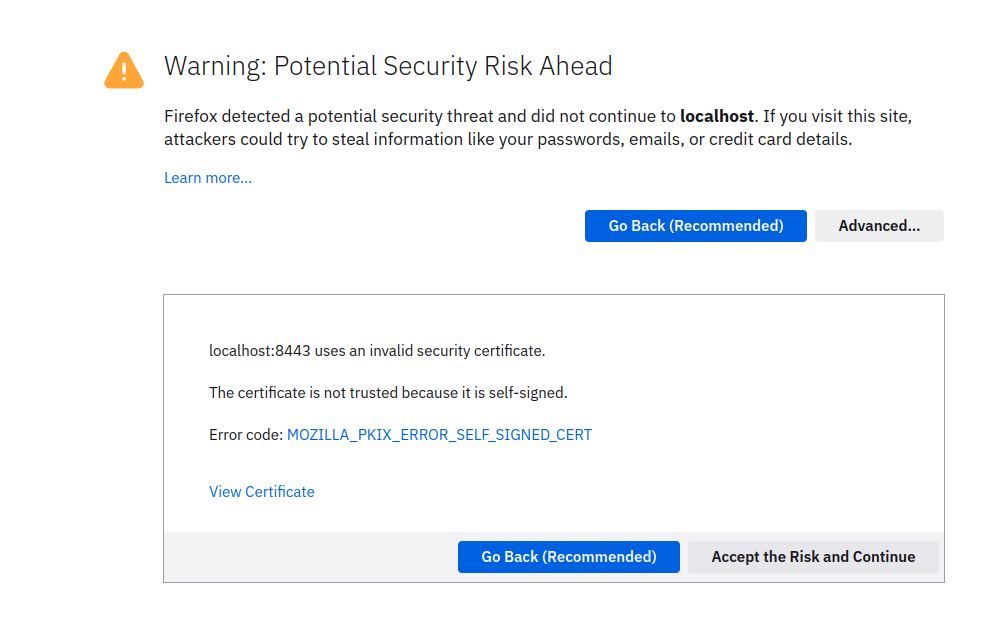
\includegraphics[width=\linewidth]{resources/firefox-warning.png}
    \end{subfigure}
    \begin{subfigure}[b]{0.3\linewidth}
        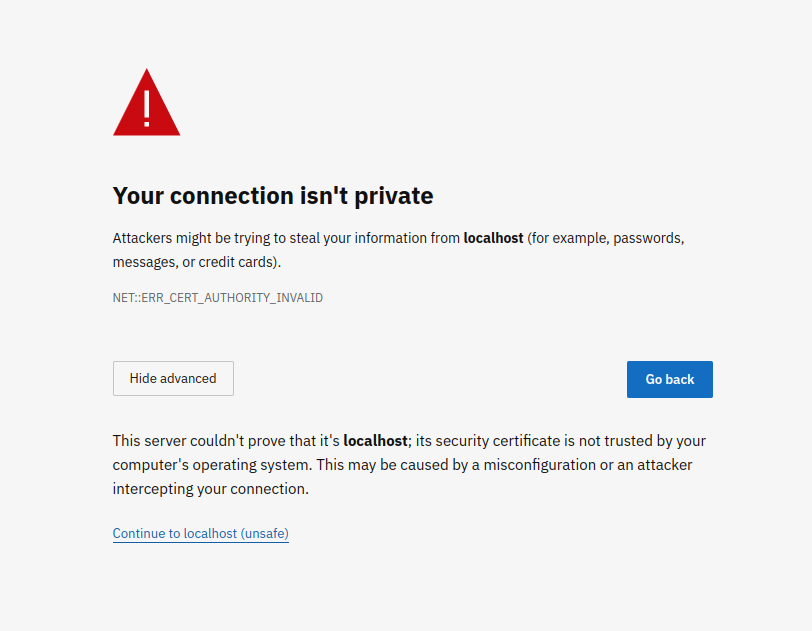
\includegraphics[width=\linewidth]{resources/edge-warning.png}
    \end{subfigure}
    \caption{Warning as presented by different browsers (Firefox on the left; Microsoft Edge on the right).}
\end{figure}

\section{Usage}

\subsection{General}

\subsubsection{Registration}

\begin{figure}[H]
    \centering
    \begin{subfigure}[b]{0.4\linewidth}
        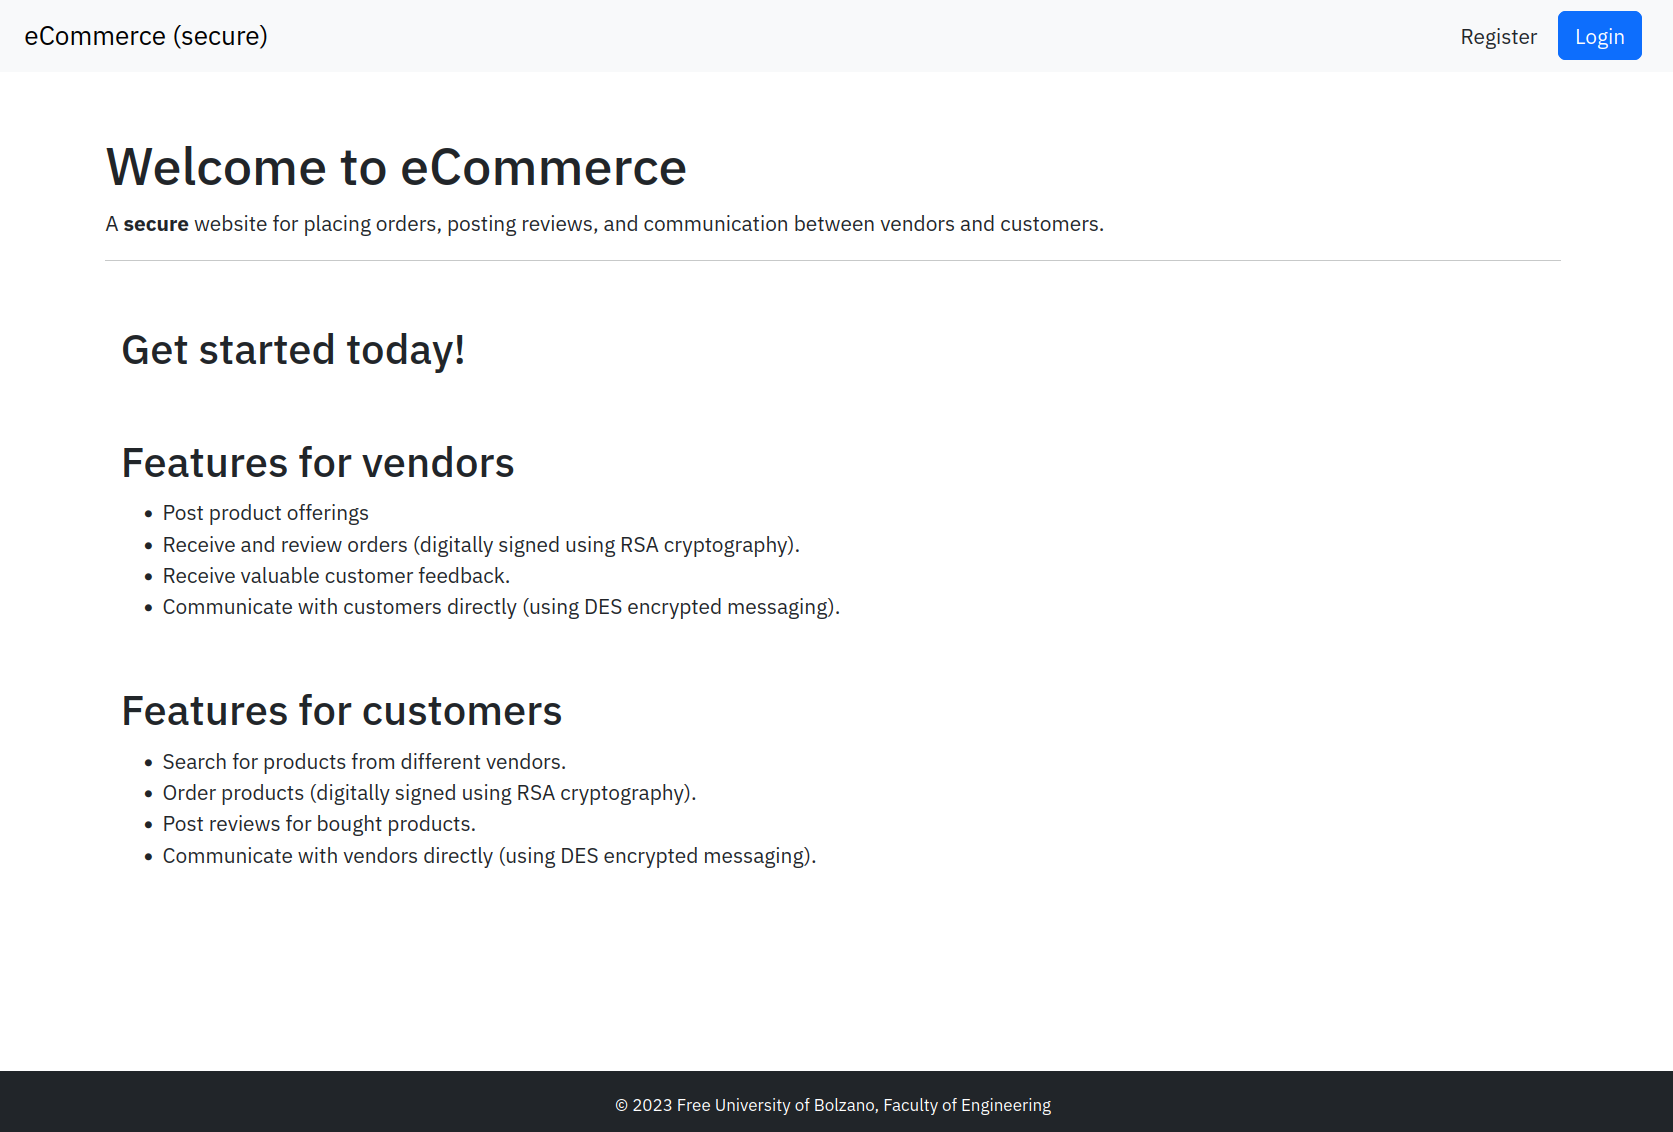
\includegraphics[width=\linewidth]{resources/welcome.png}
        \caption{The first screen presented to users.}
    \end{subfigure}
    \begin{subfigure}[b]{0.4\linewidth}
        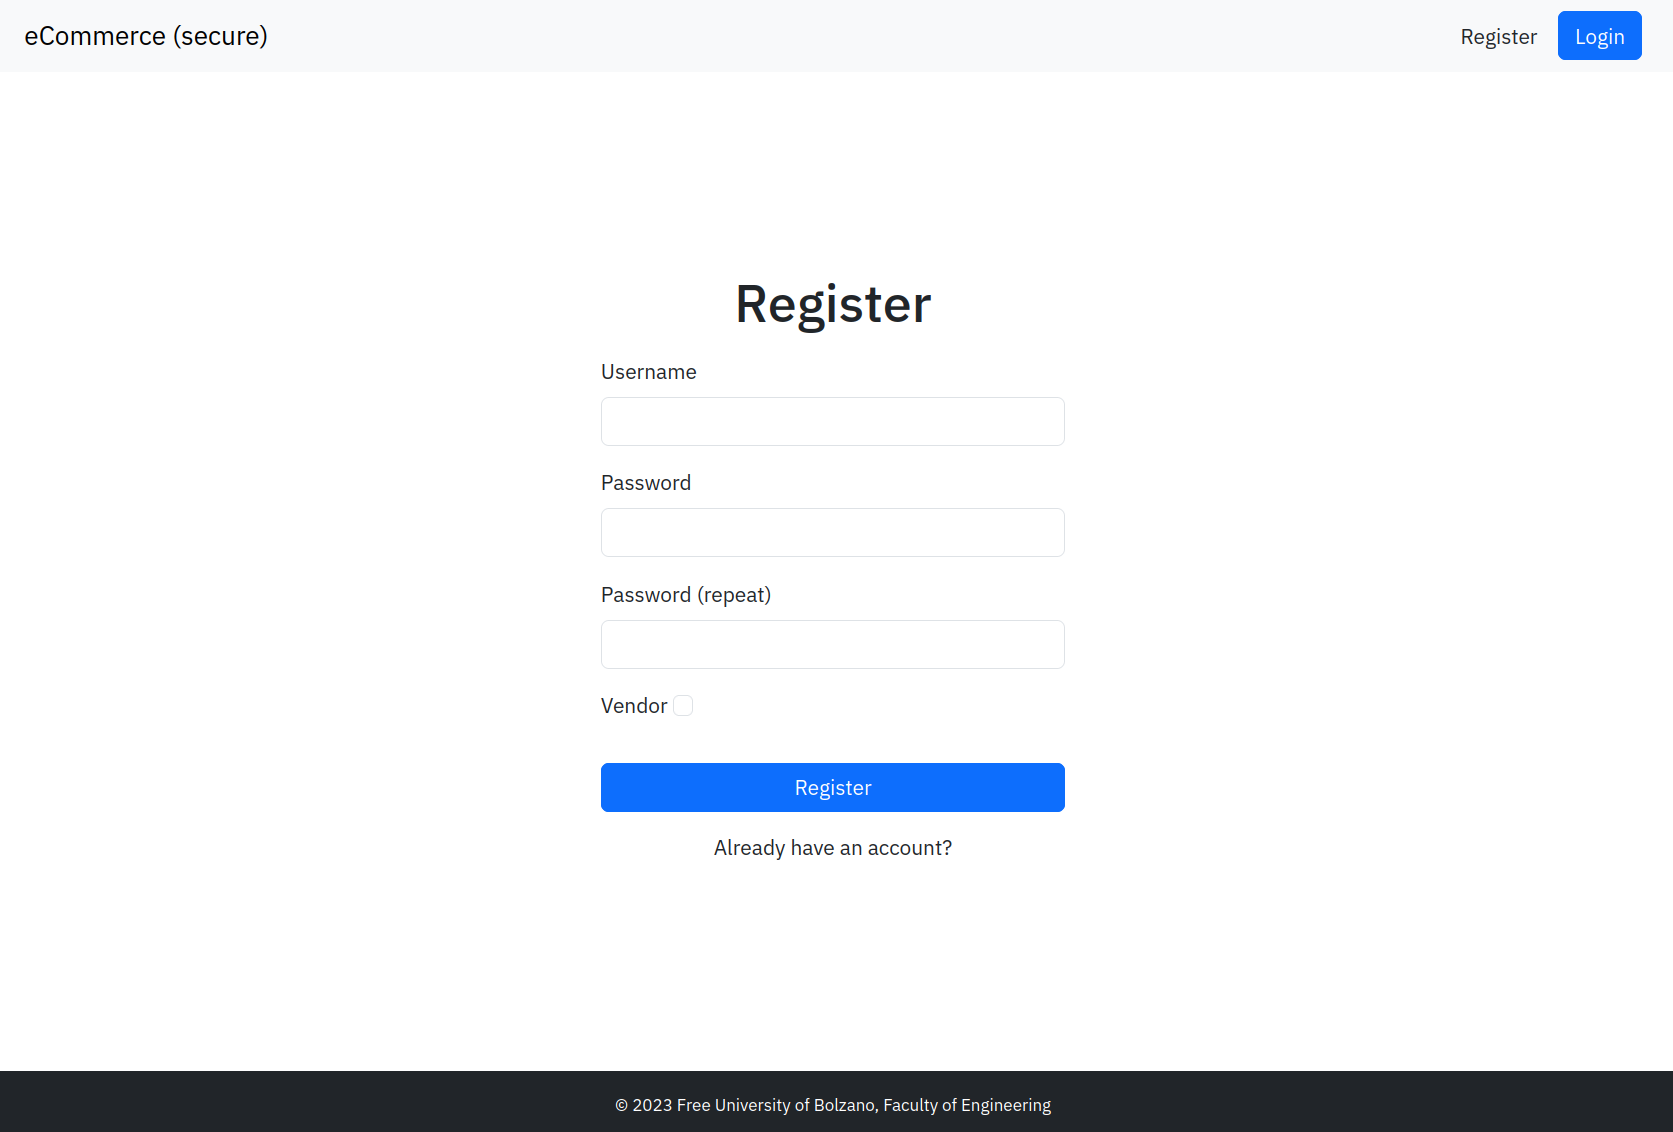
\includegraphics[width=\linewidth]{resources/register.png}
        \caption{Example of the registration form.}
    \end{subfigure}
    \caption{Example of the registration procedure.}
\end{figure}

To register, the user must supply a username containing at least 3 characters. In the secure version, aside from underscores and dots, only alphanumerical ASCII characters are permitted in usernames. The user is also asked to enter a password twice. The two repetitions of the password must match and, in the secure version, there are additional constraints on the password. Passwords in the secure version must be at least 8 characters long, contain lowercase and uppercase letters, numbers, and special characters. Usernames are unique, so if another user has already taken the desired username, registration will fail.

The user is further asked to declare whether they are a vendor or a customer. Vendors should check the checkbox at the bottom of the form labelled "Vendor". Customers and vendors have access to different functionality and the choice made during registration can not be changed later.

\subsubsection{Login}

\begin{figure}[H]
    \centering
    \begin{subfigure}[b]{0.4\linewidth}
        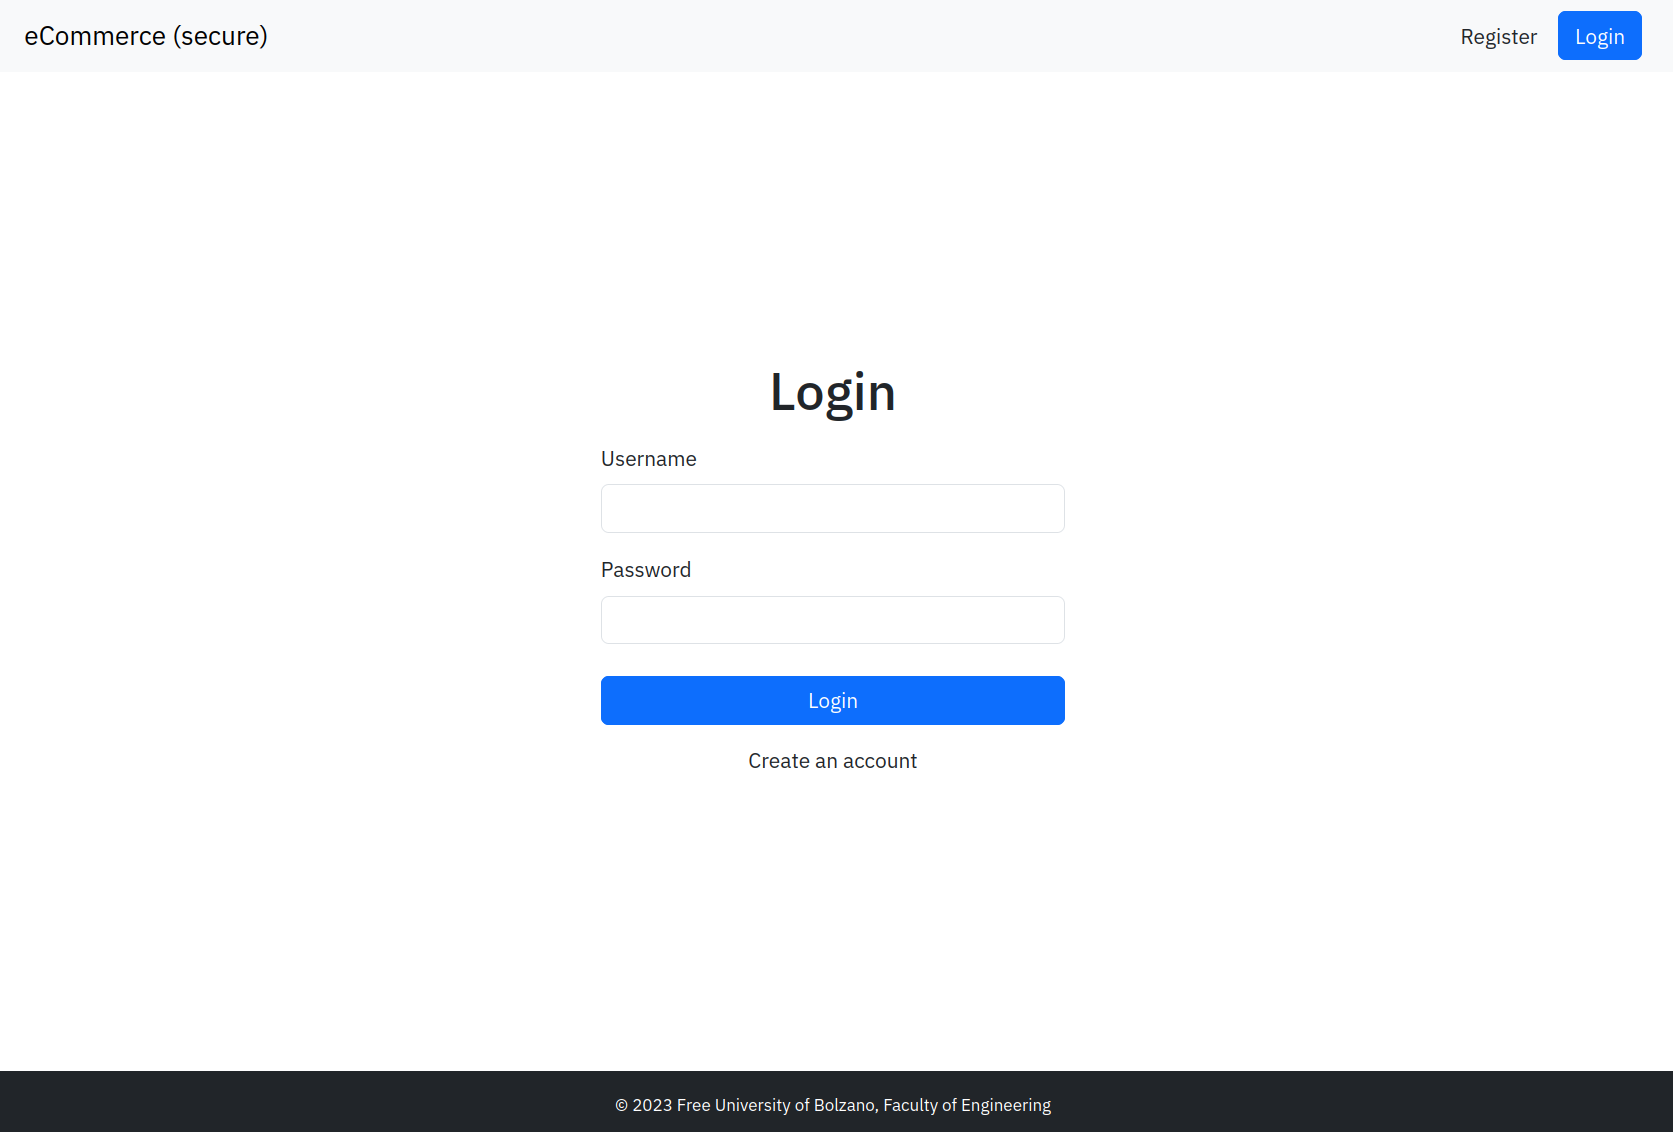
\includegraphics[width=\linewidth]{resources/login.png}
    \end{subfigure}
    \caption{Example of the login form.}
\end{figure}

If the user already has an account, they can select the “Already have an account?” button, or use the “Login” button in the header of the website. To log into the web application the user must provide username and password. If these do not match any known user, the user will not be allowed to access any other part of the application.

\subsubsection{Search and read products}

\begin{figure}[H]
    \centering
    \begin{subfigure}[b]{0.4\linewidth}
        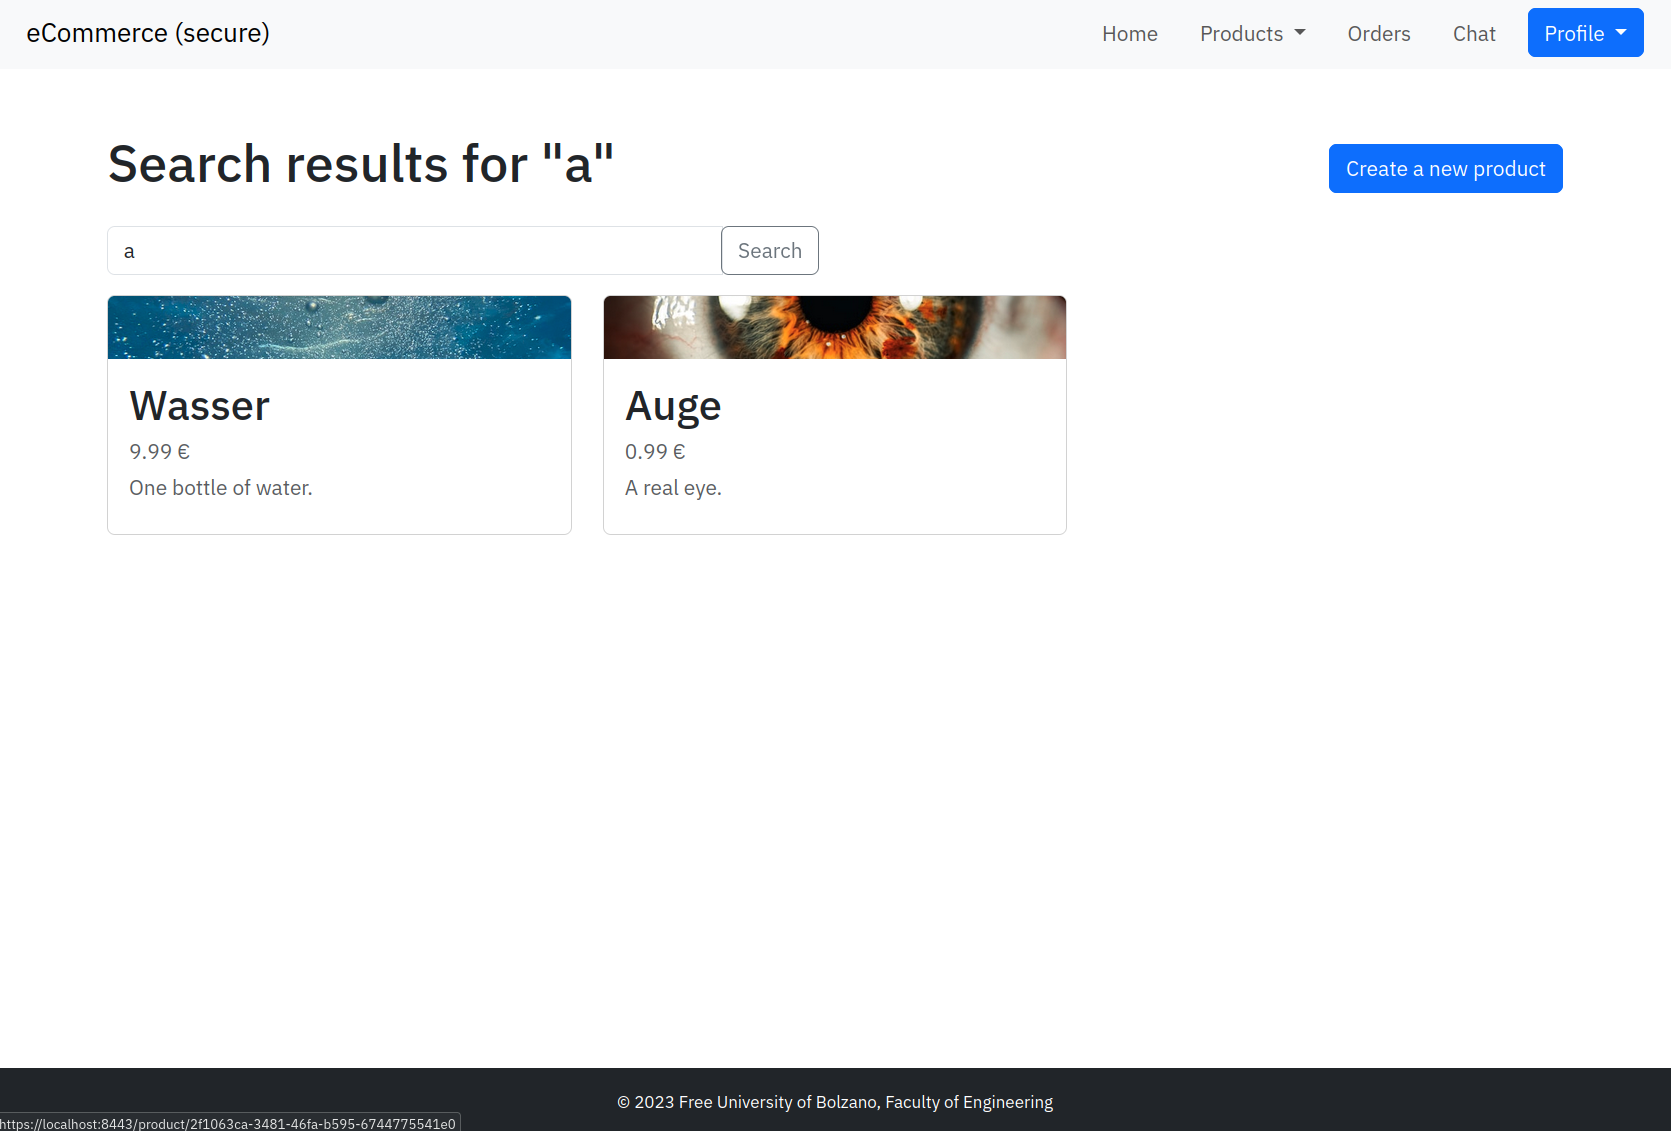
\includegraphics[width=\linewidth]{resources/seach-product.png}
        \caption{The listing of all products contained in the search.}
    \end{subfigure}
    \begin{subfigure}[b]{0.4\linewidth}
        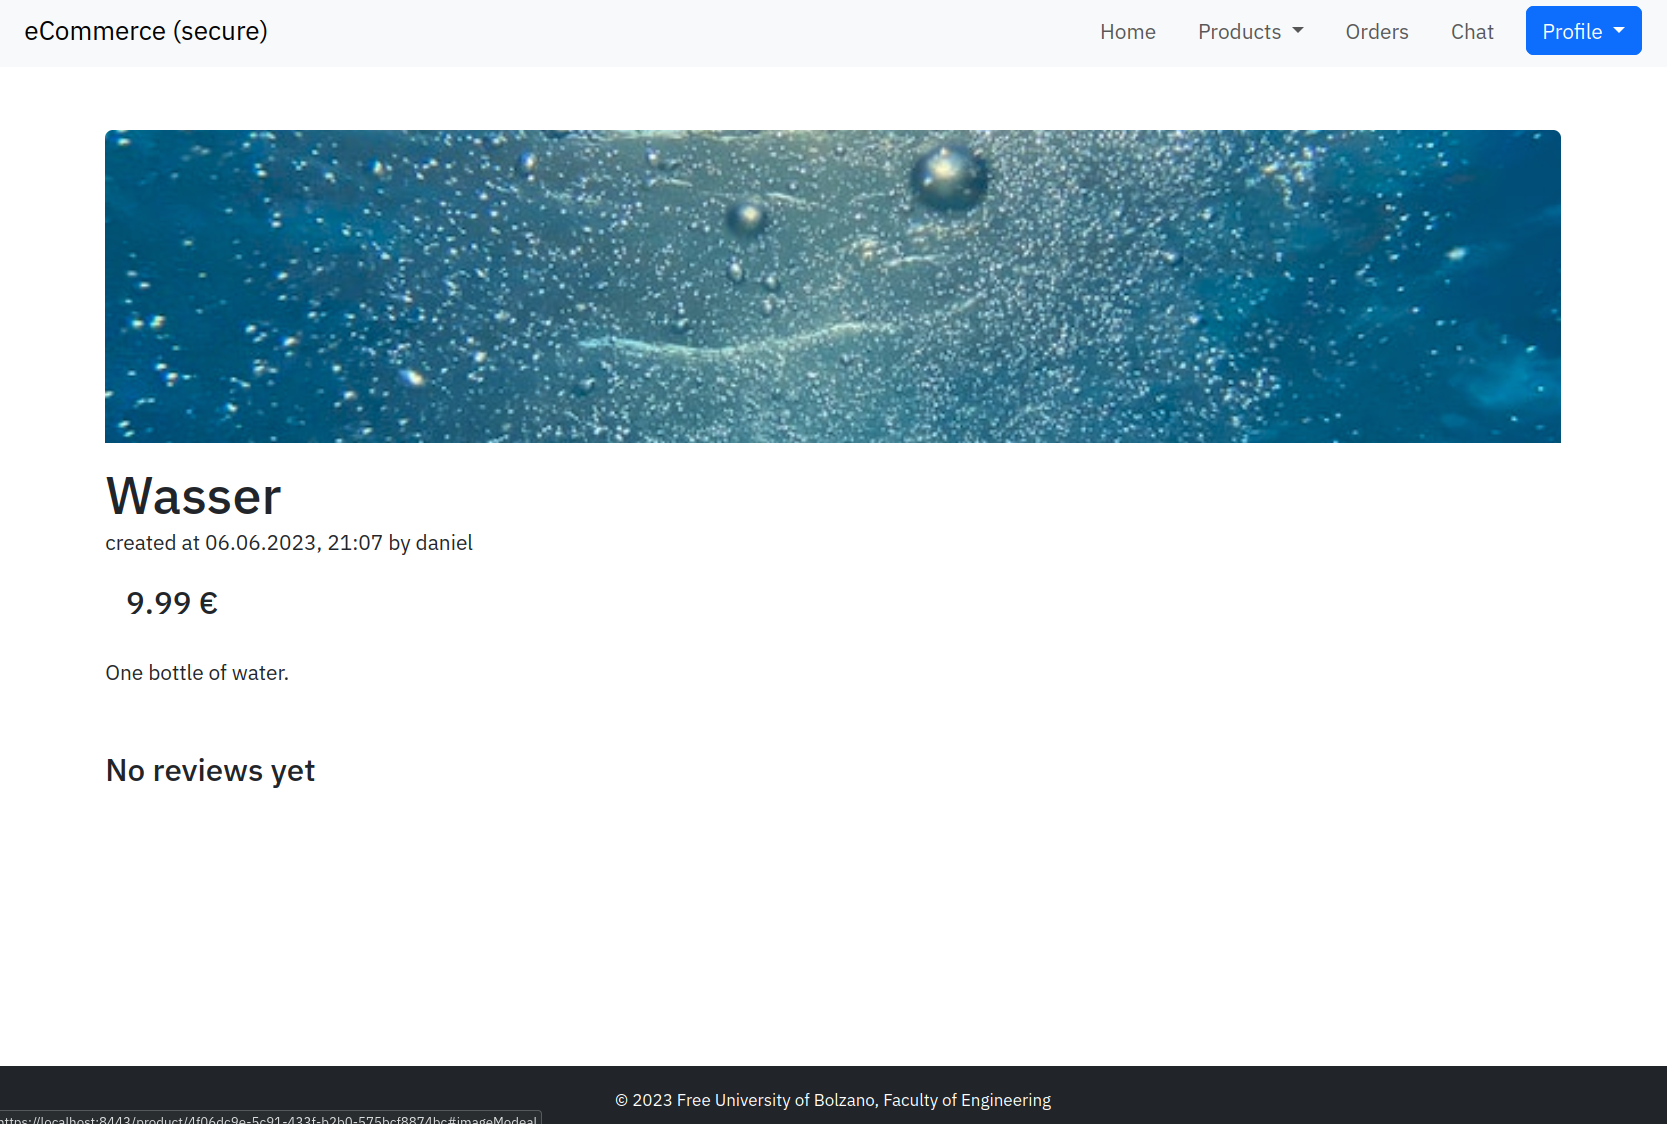
\includegraphics[width=\linewidth]{resources/product.png}
        \caption{Detailed view of one product.}
    \end{subfigure}
    \caption{Shows the process of searching and reading product cards.}
\end{figure}

To search for a product, use the search field at the beginning of the product list. The product list is accessible by using the “Products” menu in the header of the webpage. Vendors have a special version of the product list that shows only product cards posted by them under the menu item “My products”. To see further details on a single product, select it in the list of products by clicking on the product card. This is also the section in which reviews for products and relies to those reviews are made visible.


\subsection{Vendors}

\subsubsection{Post product}

\begin{figure}[H]
    \centering
    \begin{subfigure}[b]{0.4\linewidth}
        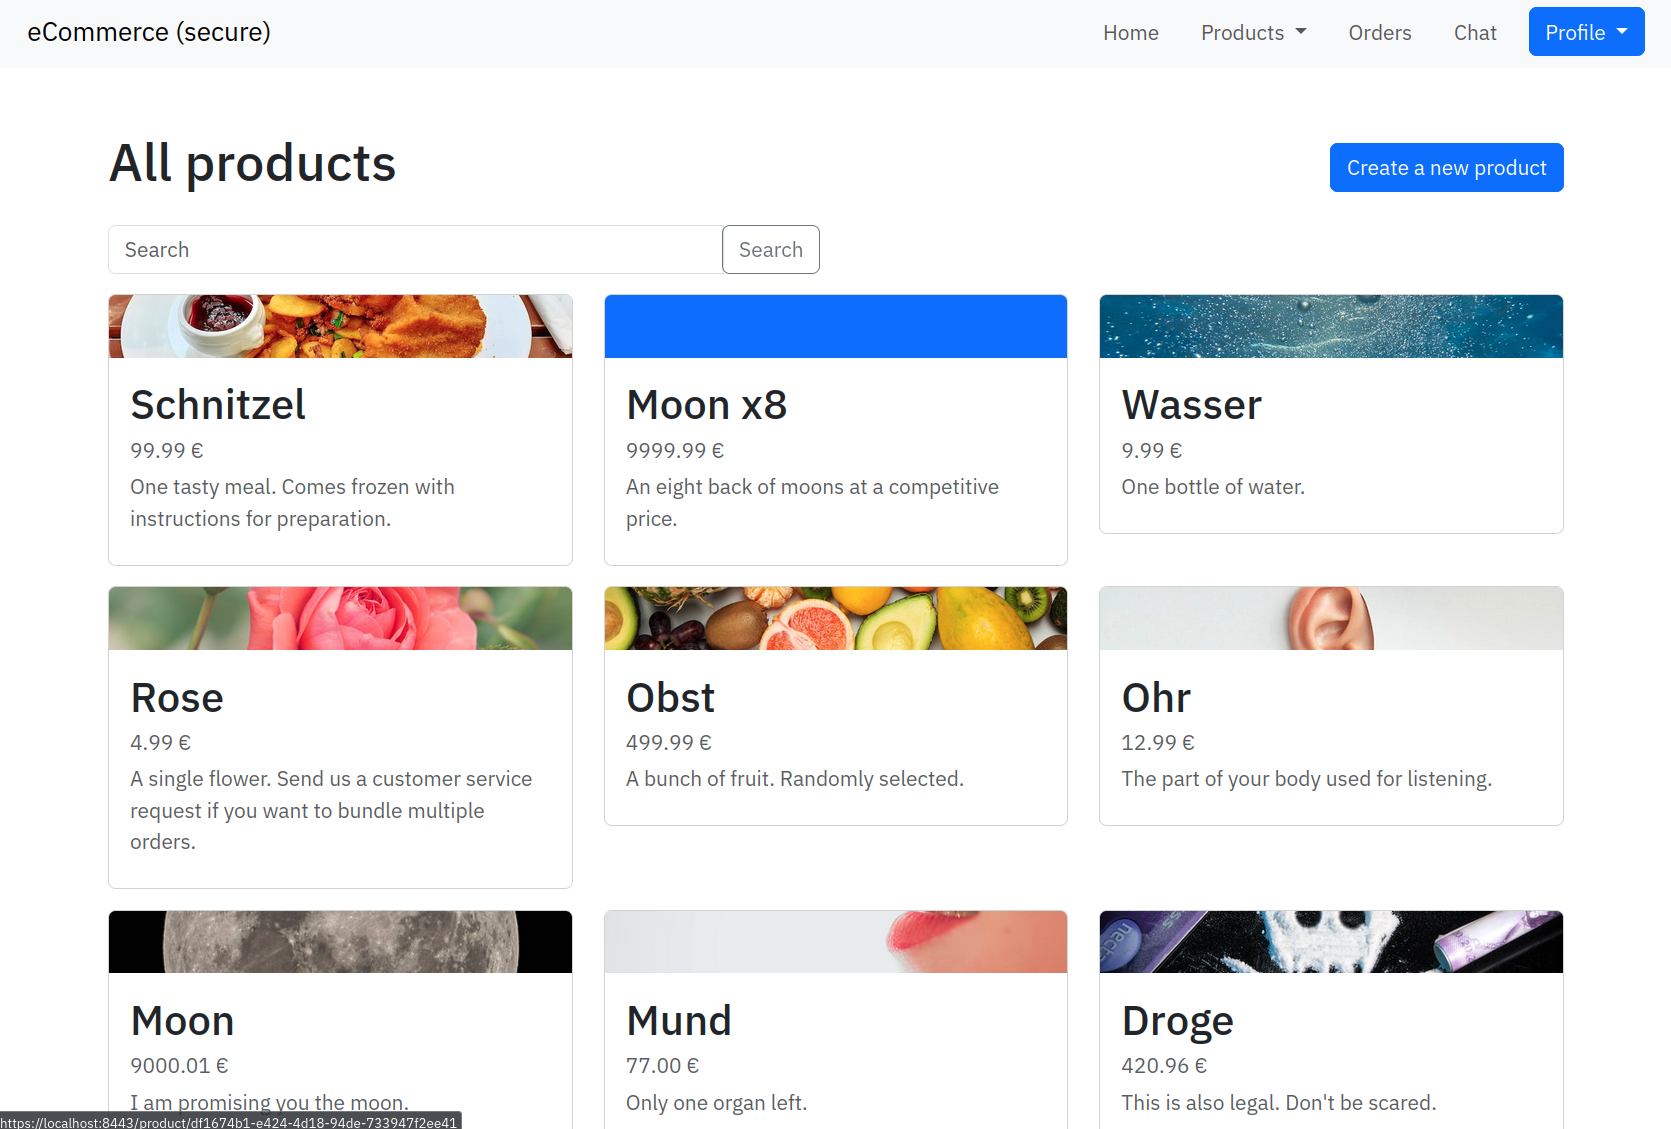
\includegraphics[width=\linewidth]{resources/products.png}
        \caption{The listing of all products currently posted.}
    \end{subfigure}
    \begin{subfigure}[b]{0.4\linewidth}
        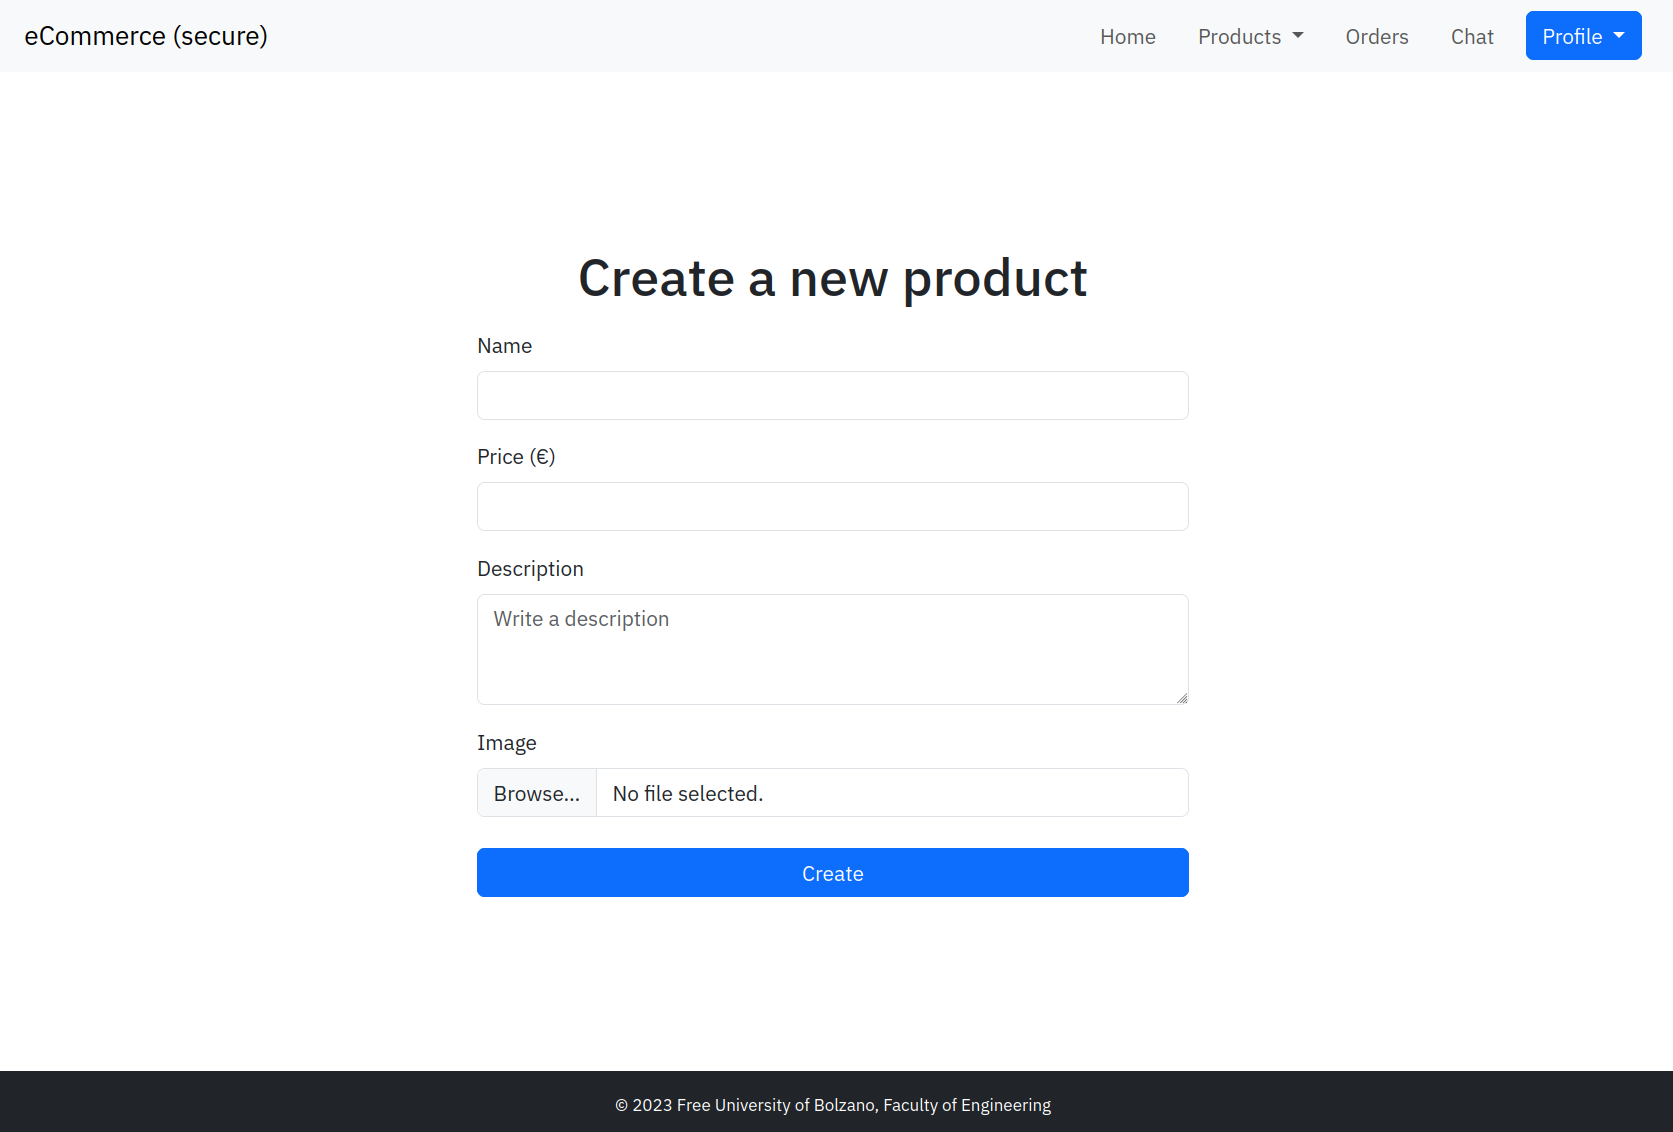
\includegraphics[width=\linewidth]{resources/new-product.png}
        \caption{Example of the form for creating new product posts.}
    \end{subfigure}
    \caption{Example of the steps for creating a new product.}
\end{figure}

New products can be posted by vendors by navigating to one of the product lists through the “Products” menu in the header of the webpage and then selecting “Create a new product”. The user will be presented with a form that requests a product name, price, description, and image. Both the product name and the price are mandatory, while the description and image may optionally be left blank.

\subsubsection{Check orders}

\begin{figure}[H]
    \centering
    \begin{subfigure}[b]{0.4\linewidth}
        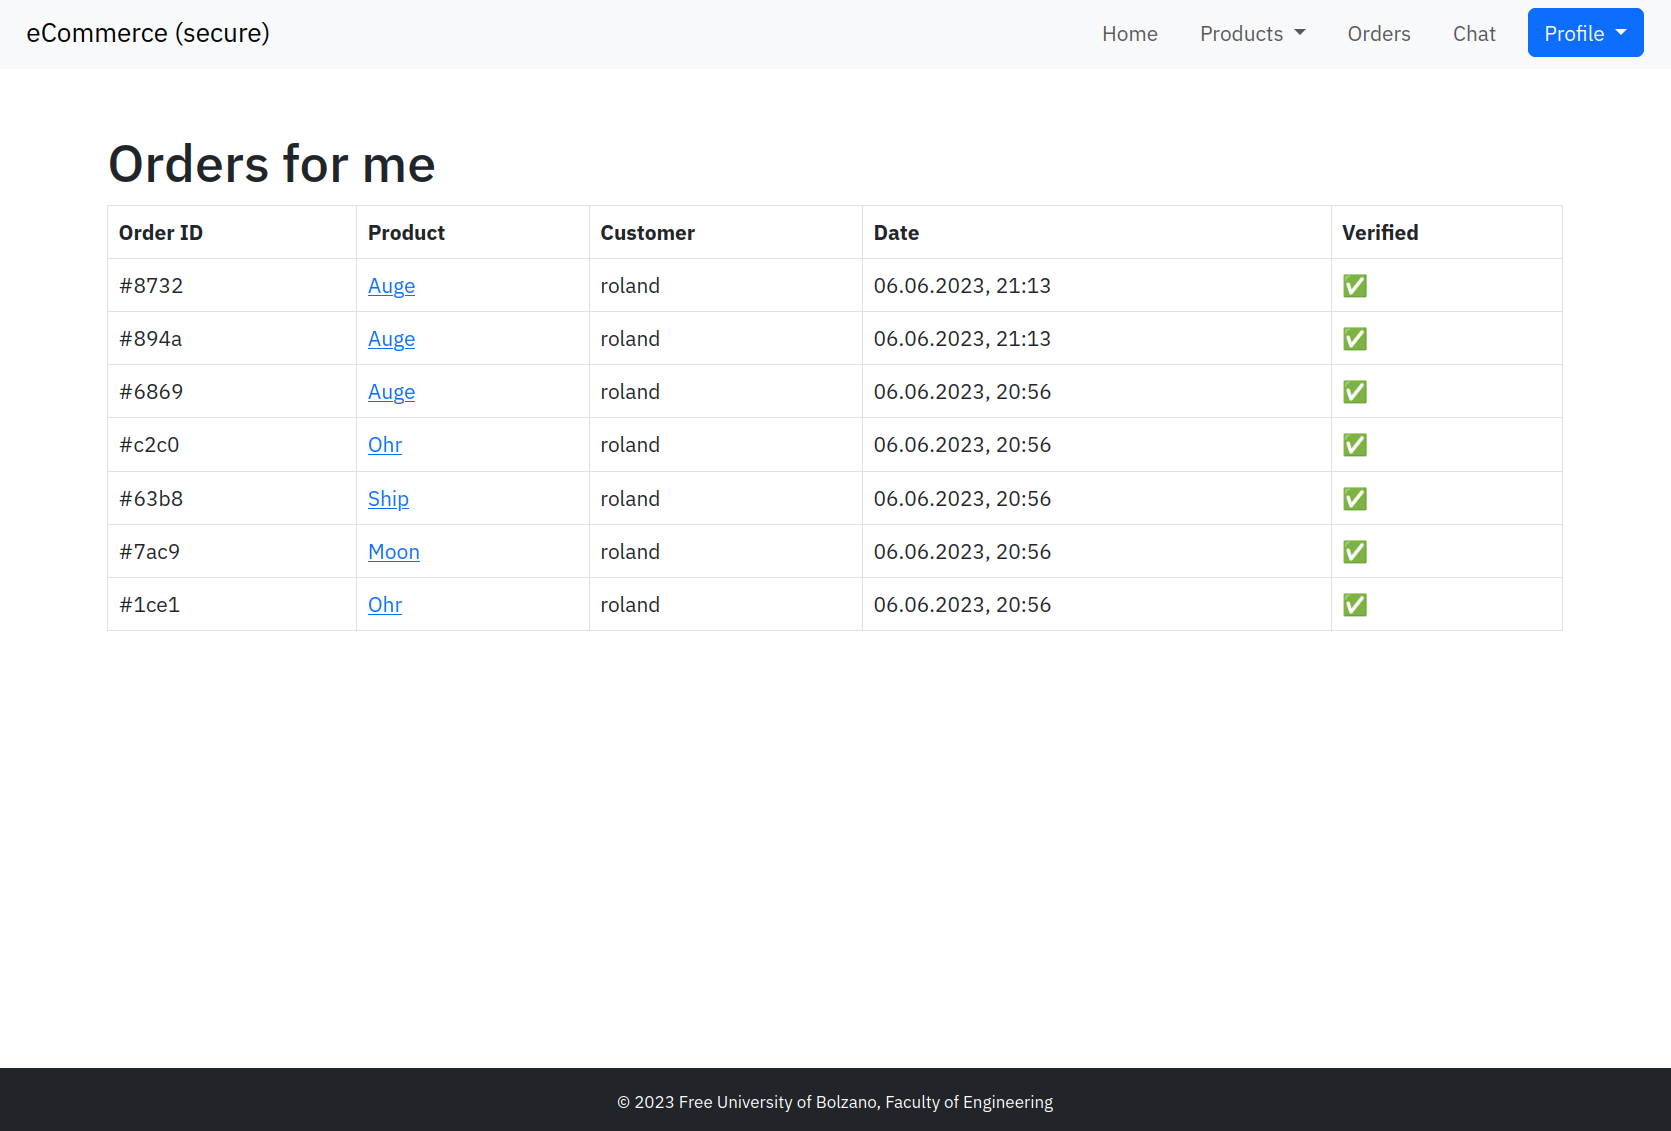
\includegraphics[width=\linewidth]{resources/orders.png}
    \end{subfigure}
    \caption{Example showing the list of orders for a vendors products.}
\end{figure}

A vendor can check the incoming orders from his customers by navigating to the orders view using the “Orders” button of the top navigation bar. For each order an order identifier, the product purchased, the customer that performed the purchase, and the data of purchase are displayed. Additionally, the secure version of the application also features support for digital signatures of the order documents. If the order has a valid signature in the database, a check mark will be displayed. If no signature is present, or it is somehow invalid, a red x-mark will be shown for that order.

\subsubsection{Reply to reviews}

\begin{figure}[H]
    \centering
    \begin{subfigure}[b]{0.4\linewidth}
        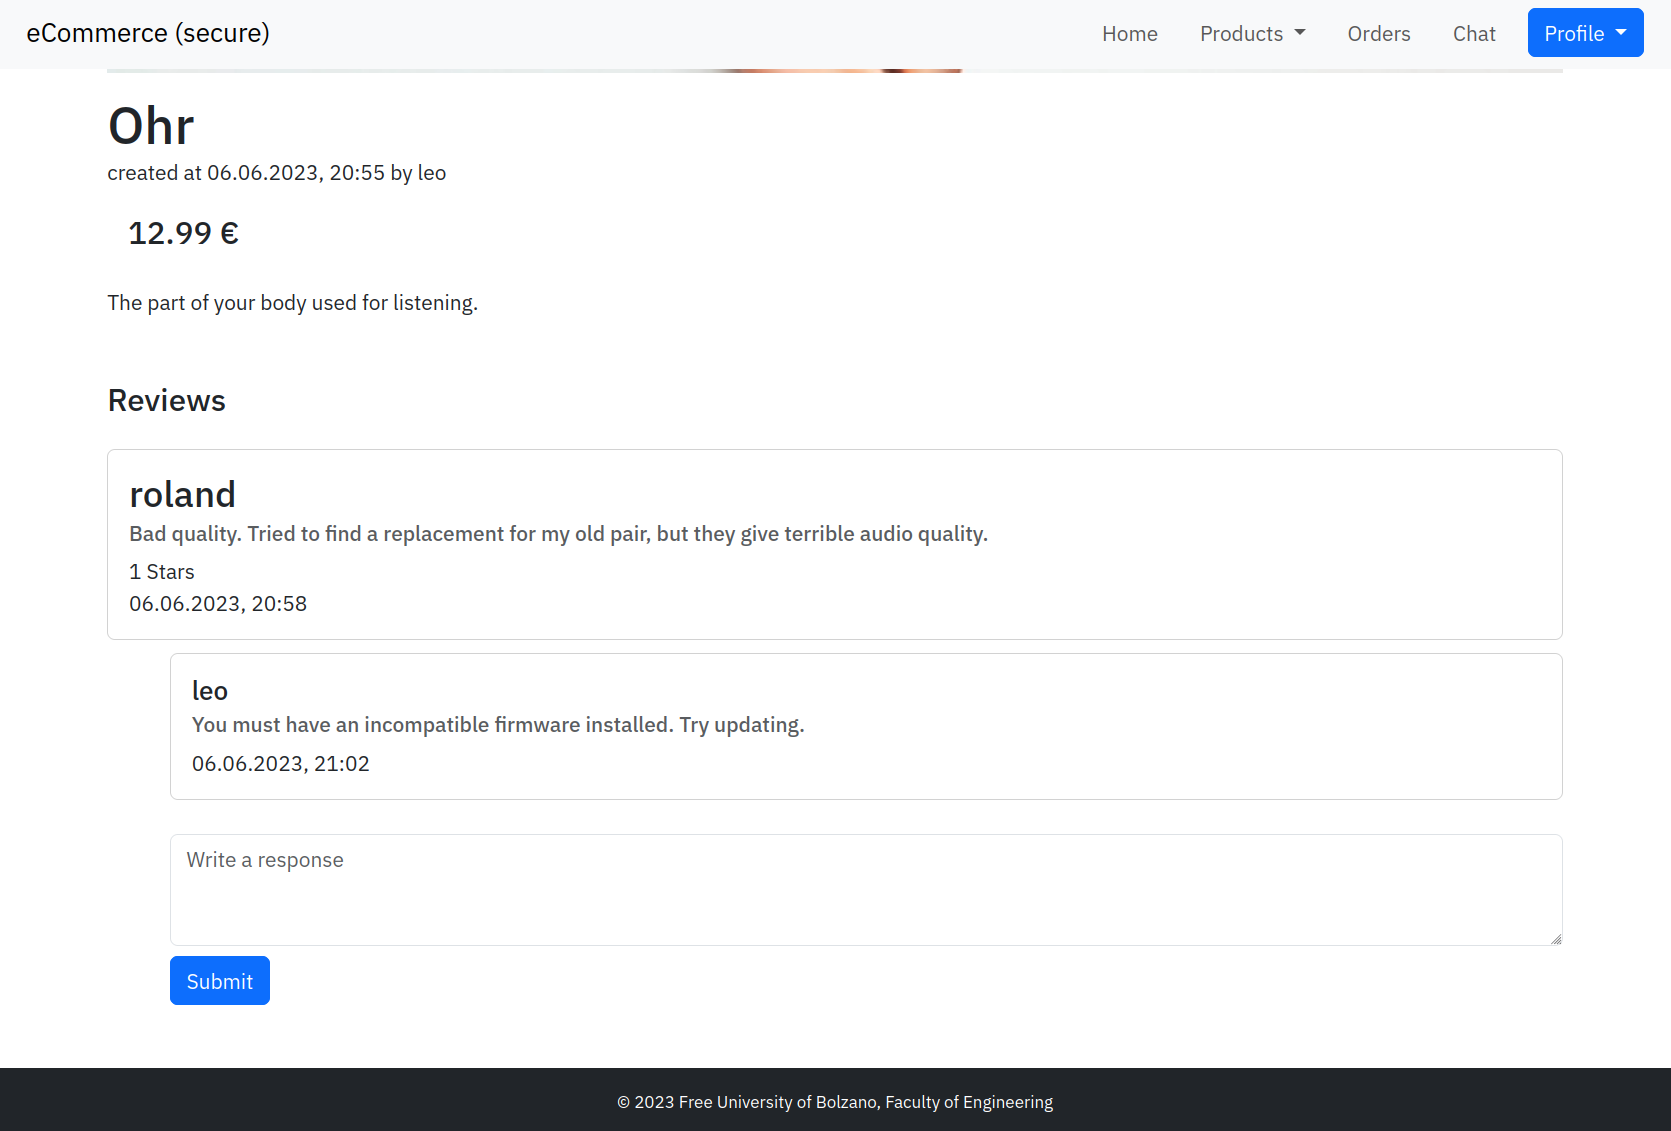
\includegraphics[width=\linewidth]{resources/response.png}
    \end{subfigure}
    \caption{Example showing the way vendors can reply to reviews.}
\end{figure}

If a customer has posted a review for a product of a vendor, that vendor can reply to the review. This is possible by navigating to the product information page and writing the response in the text field underneath the review. To post the reply press the “Submit” button underneath the text area.

\subsubsection{Chat with customers}

\begin{figure}[H]
    \centering
    \begin{subfigure}[b]{0.4\linewidth}
        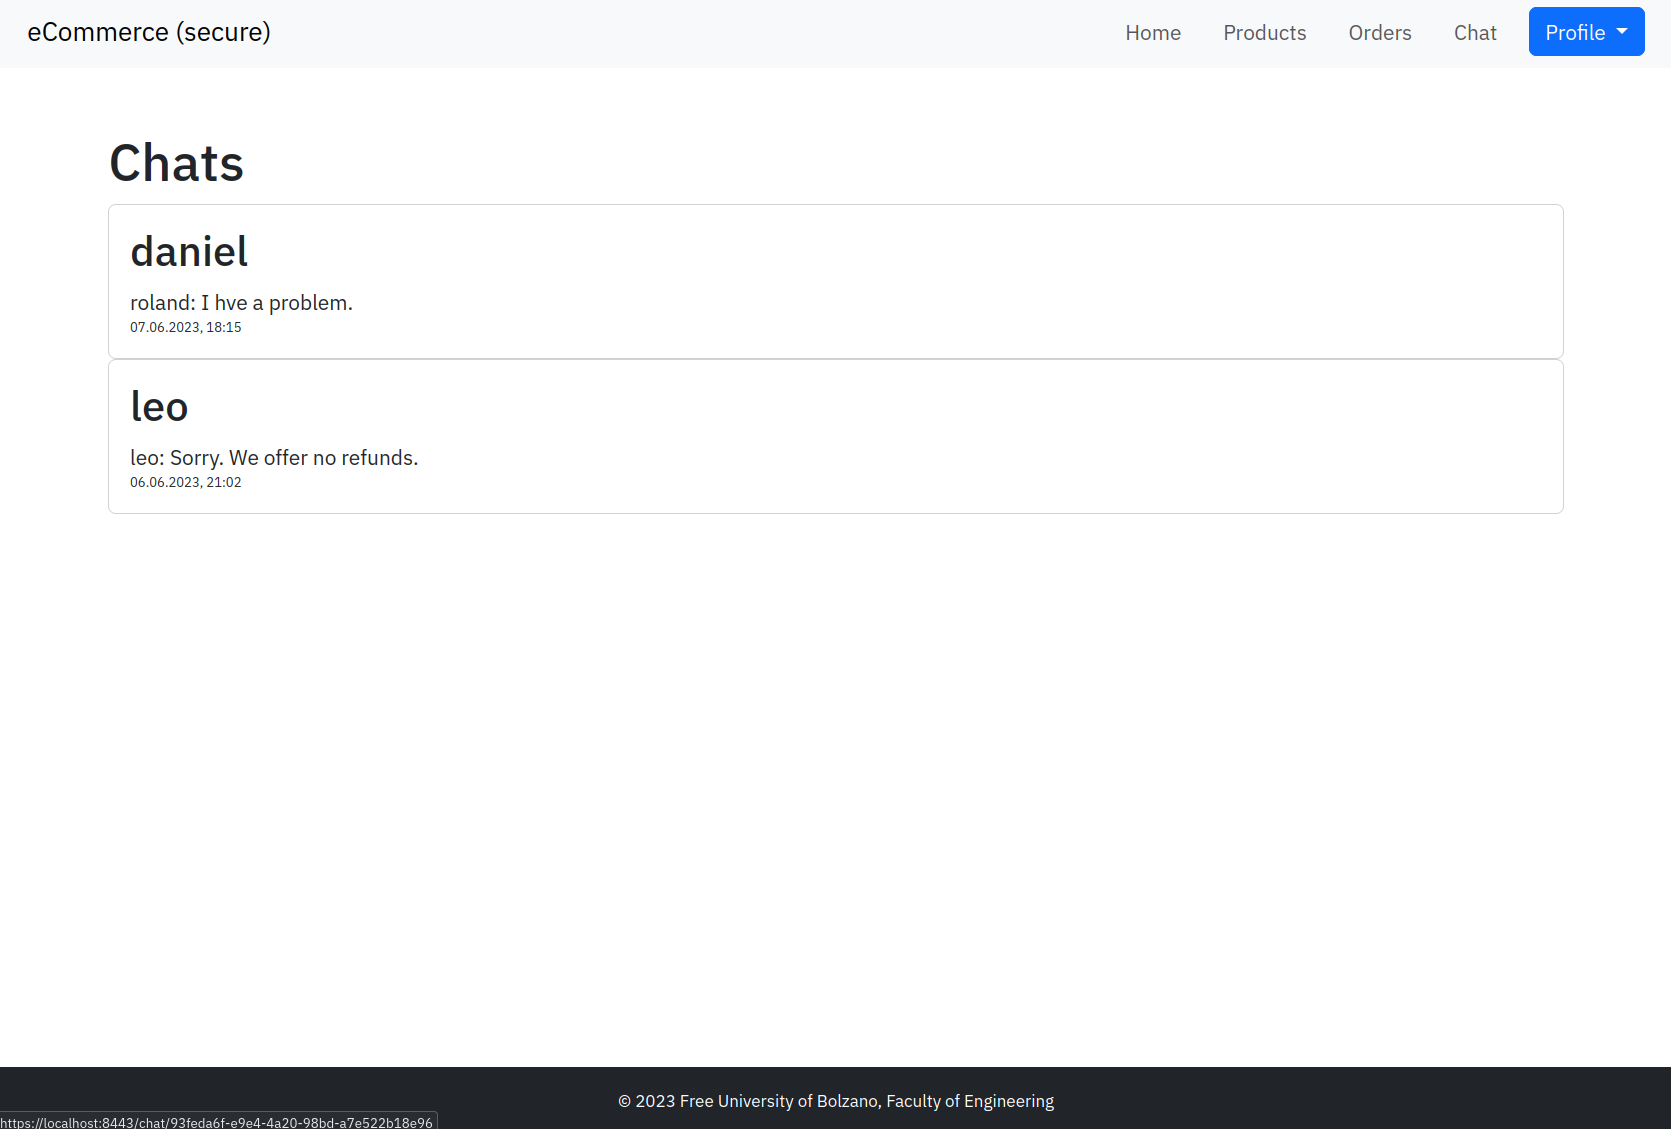
\includegraphics[width=\linewidth]{resources/chat-list.png}
        \caption{List of all user the vendor has communicated with.}
    \end{subfigure}
    \begin{subfigure}[b]{0.4\linewidth}
        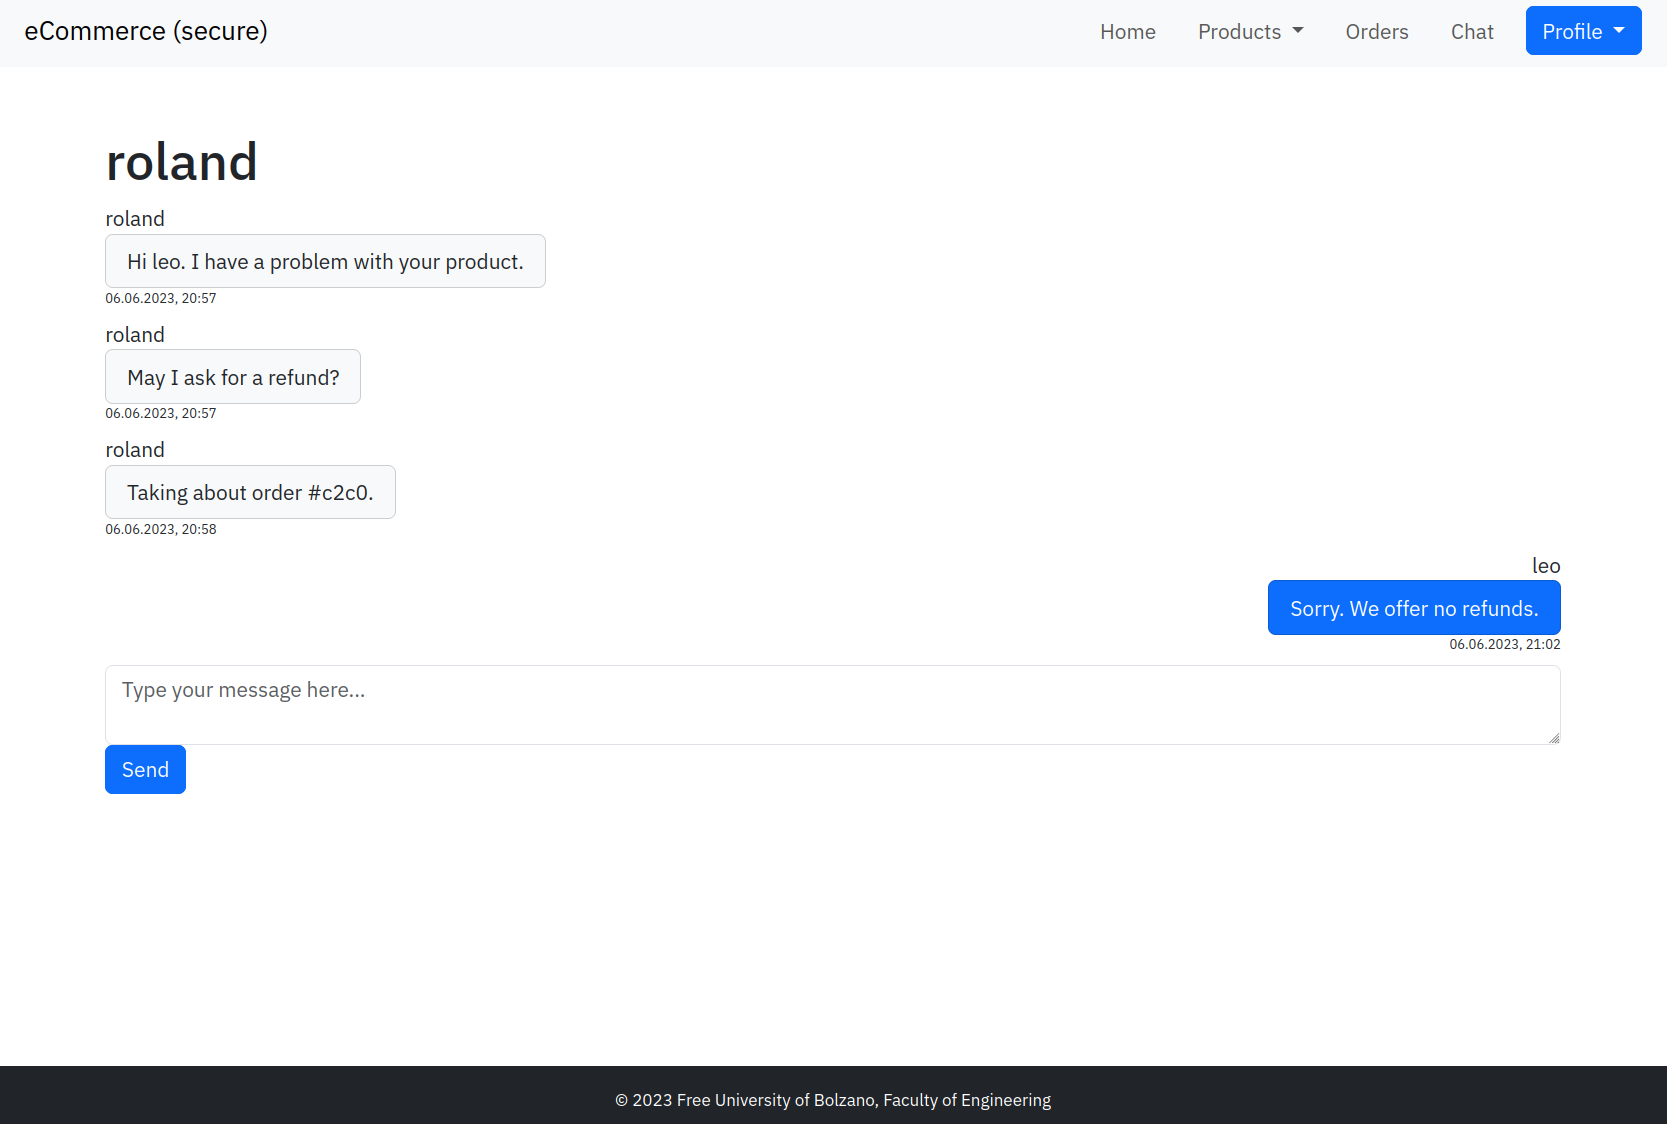
\includegraphics[width=\linewidth]{resources/chat.png}
        \caption{An example chat with a client.}
    \end{subfigure}
    \caption{Example showing how vendors can chat with customers.}
\end{figure}

The application offers the customers the ability to message vendors over a private chat. The vendor can see all users which whom they have exchanged chat messages by navigating to the chat list using the “Chats” button in the menu at the top of the page. By selecting one of the chats, the user is able to type a message into the text area at the bottom of the page and click “Send” to send me message. Messages are stored encrypted using the DES algorithm and are not accessible to anyone but the users participating in the communication.


\subsection{Customers}

\subsubsection{Buy products}

\begin{figure}[H]
    \centering
    \begin{subfigure}[b]{0.4\linewidth}
        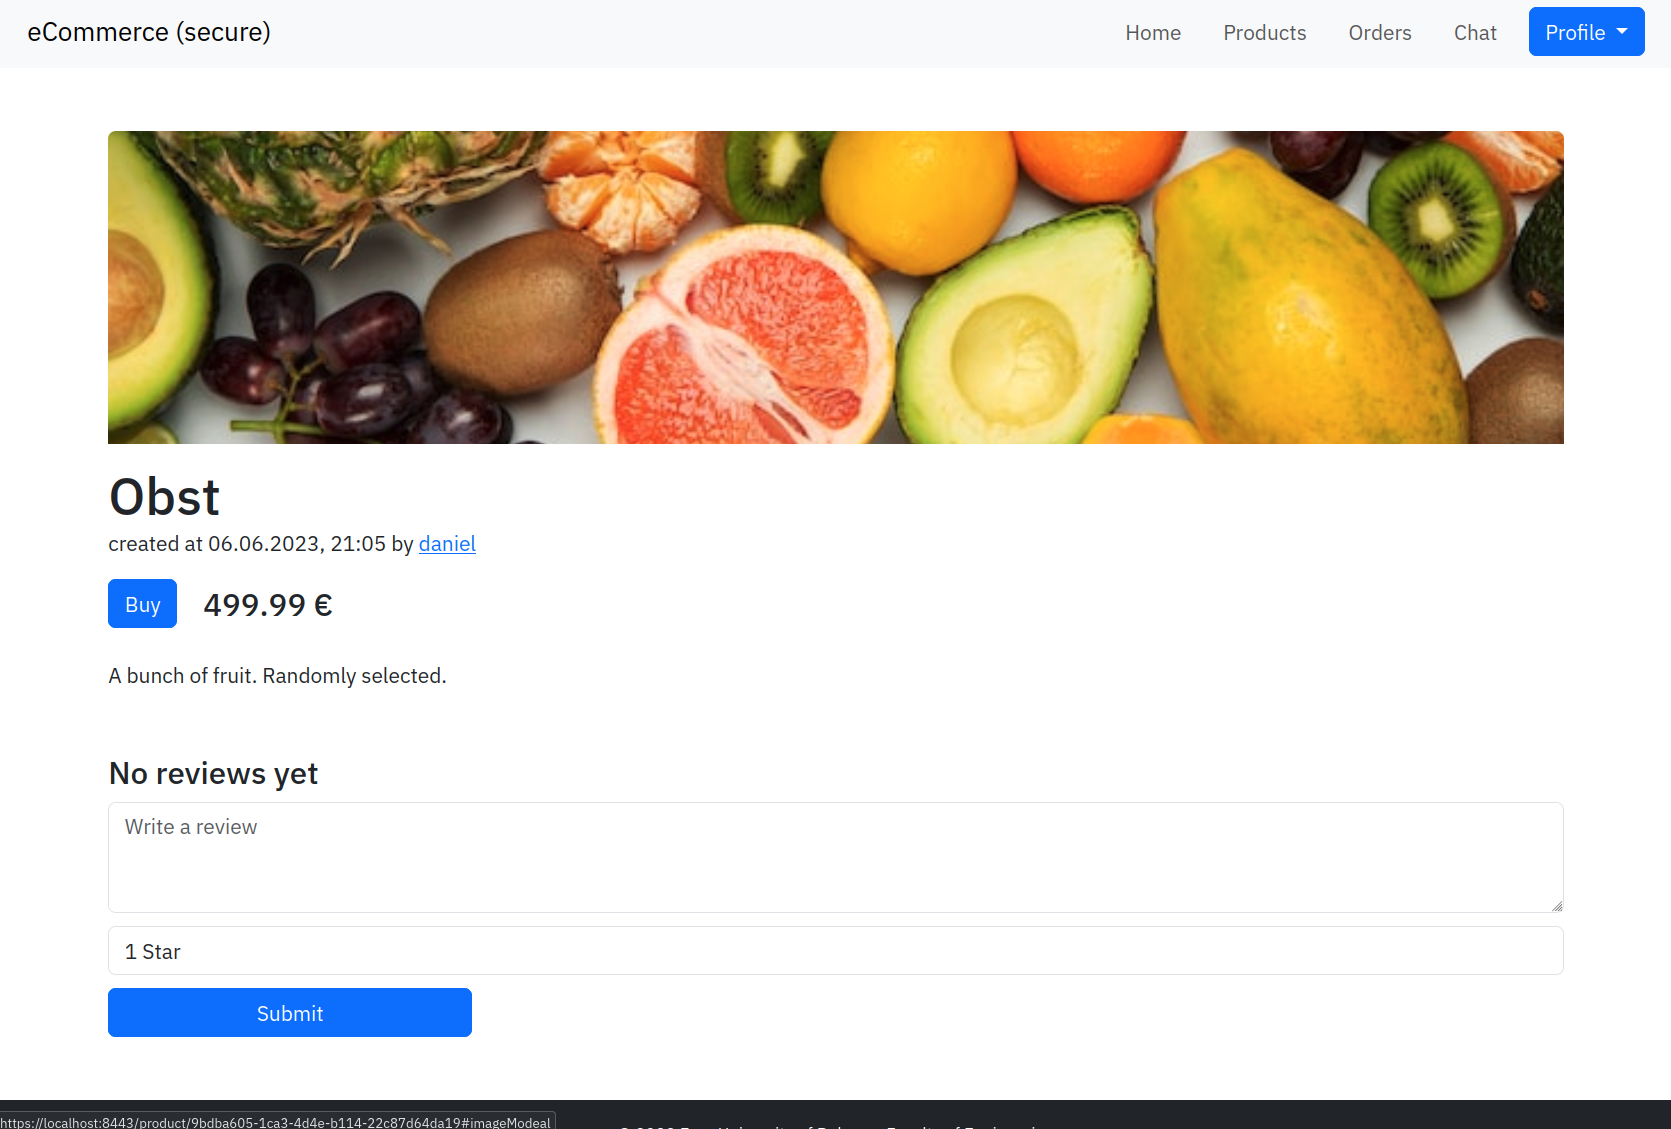
\includegraphics[width=\linewidth]{resources/product-customer.png}
        \caption{The product details page for a customer.}
    \end{subfigure}
    \begin{subfigure}[b]{0.4\linewidth}
        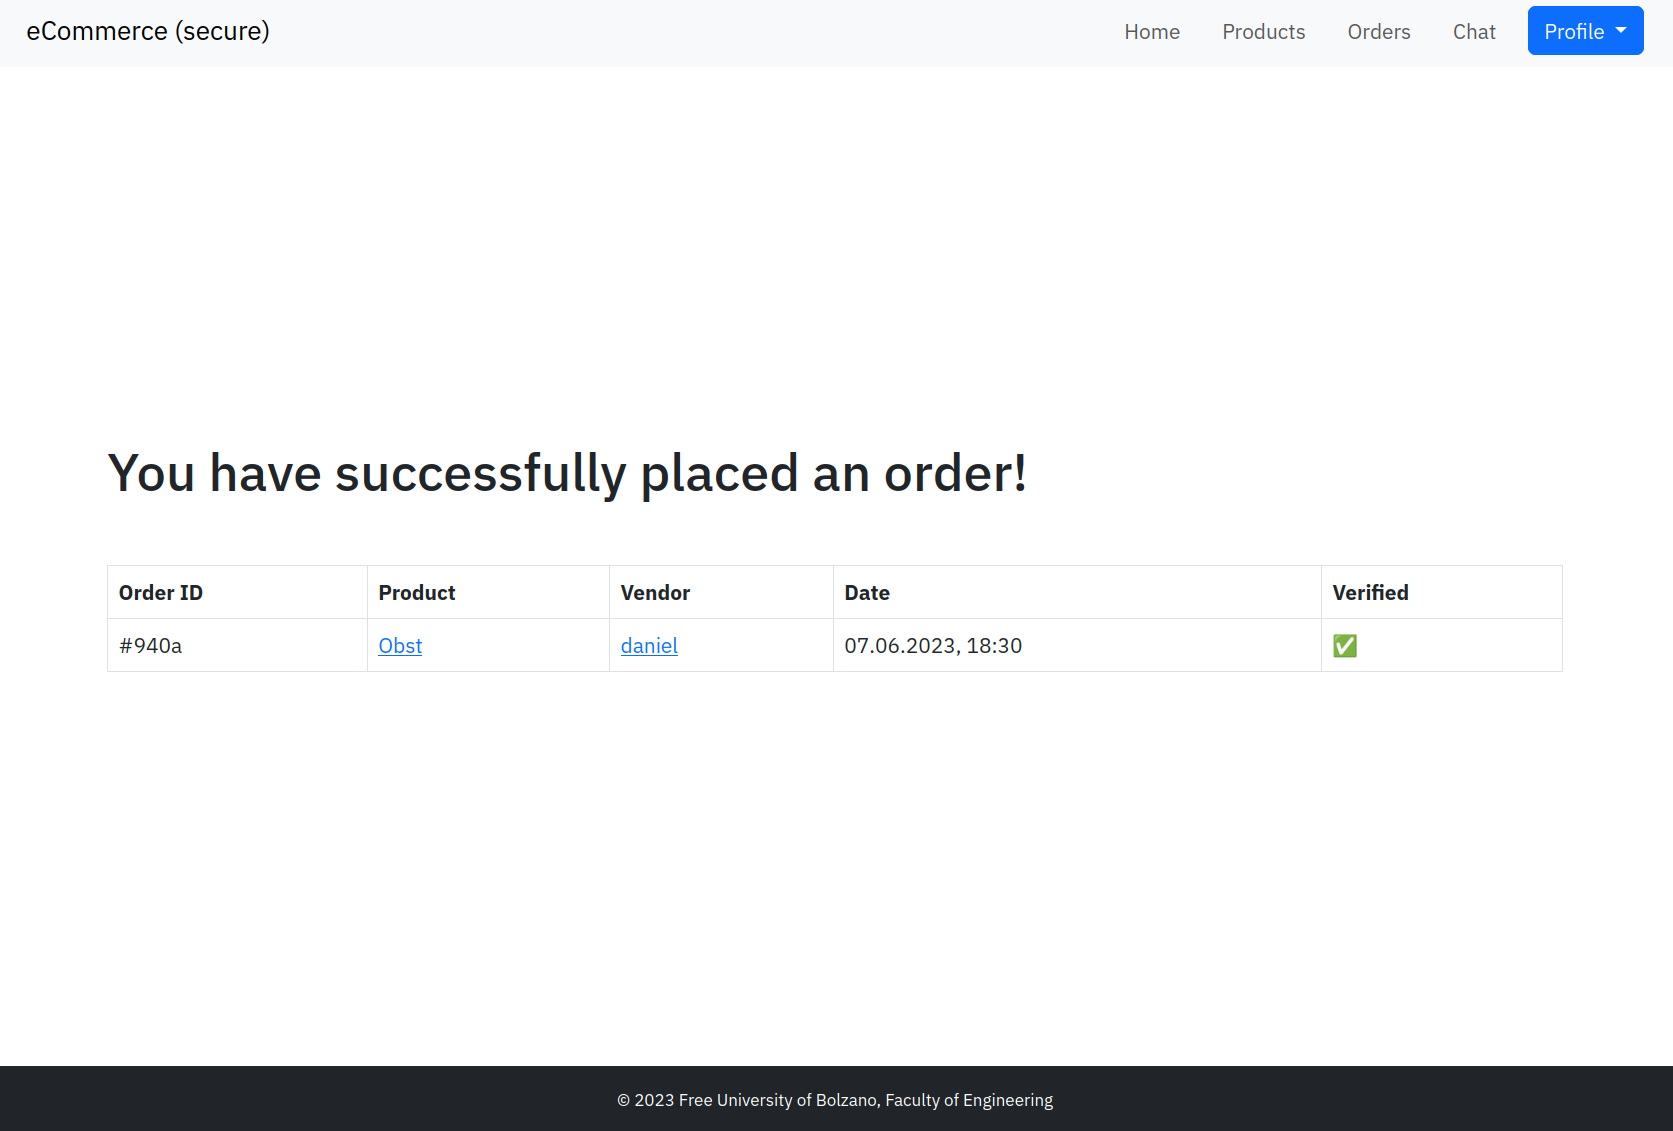
\includegraphics[width=\linewidth]{resources/order.png}
        \caption{Example of the page displayed after placing an order.}
    \end{subfigure}
    \caption{Example of how a customer can place an order.}
\end{figure}

To place an order for a product, a customer can navigate to the products details page. From there, a customer is able to by a product using the "Buy" button above the description of the product. After placing an order, a confirmation page will be displayed, showing also the information for the ordering document and, for the secure version, whether it was successfully signed with a digital signature.

\subsubsection{Post reviews}

\begin{figure}[H]
    \centering
    \begin{subfigure}[b]{0.4\linewidth}
        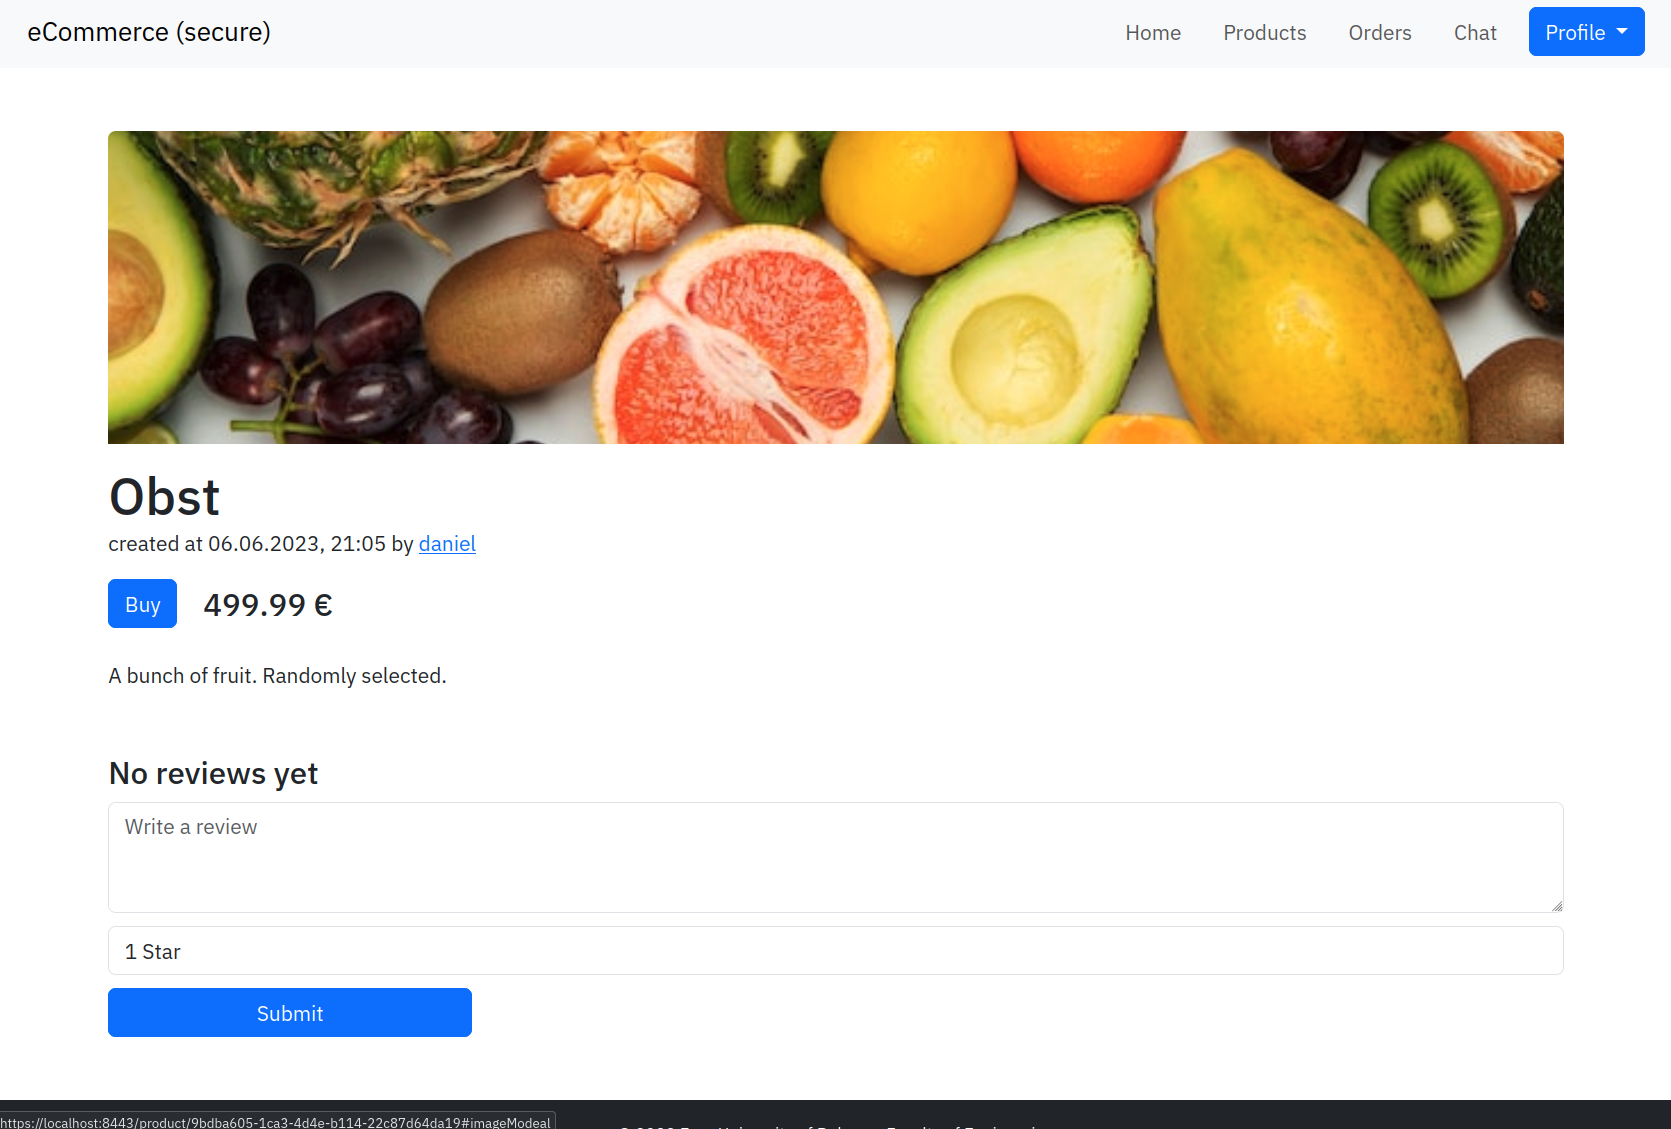
\includegraphics[width=\linewidth]{resources/product-customer.png}
    \end{subfigure}
    \caption{Example of a product page where users can post reviews.}
\end{figure}

After a user has bought a product, the product details page will show the option to post a review. Using the text area at the beginning of the reviews list, selecting a 1-5 start rating, and clicking the “Submit” button, a review can be posted.

\subsubsection{Chat with vendors}

\begin{figure}[H]
    \centering
    \begin{subfigure}[b]{0.4\linewidth}
        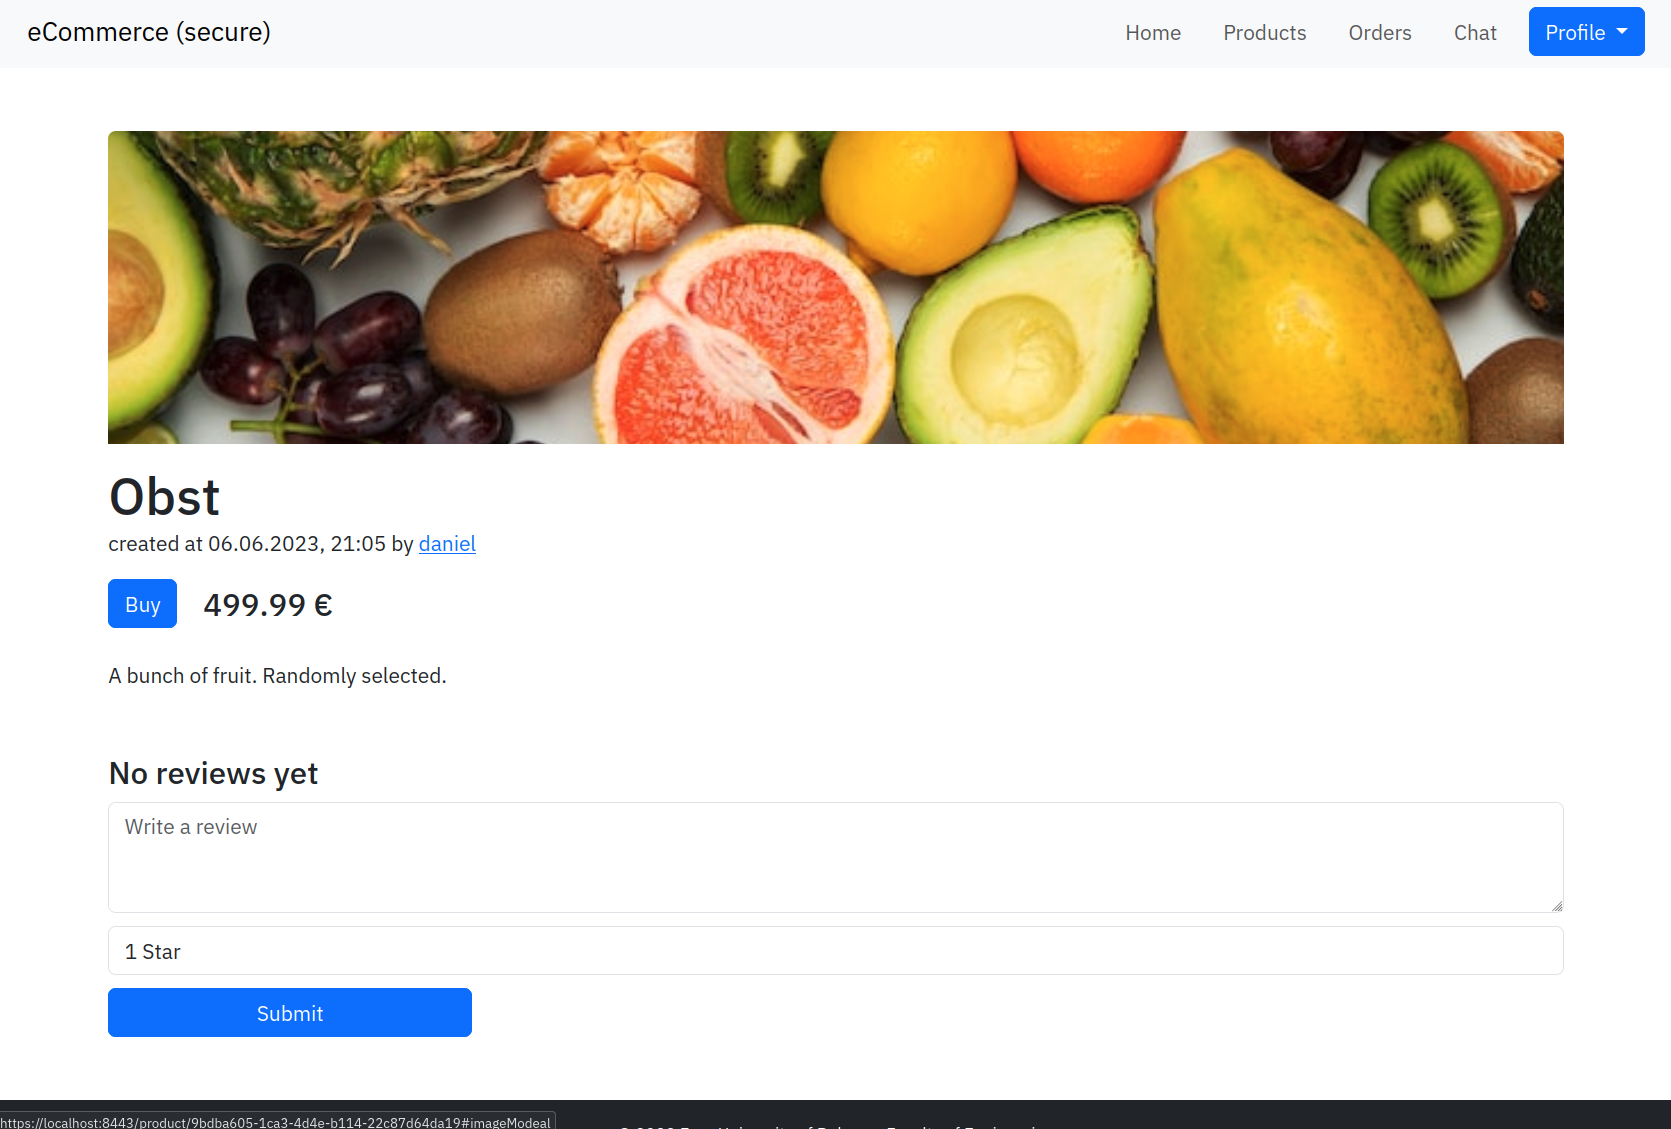
\includegraphics[width=\linewidth]{resources/product-customer.png}
        \caption{The product details page for a customer.}
    \end{subfigure}
    \begin{subfigure}[b]{0.4\linewidth}
        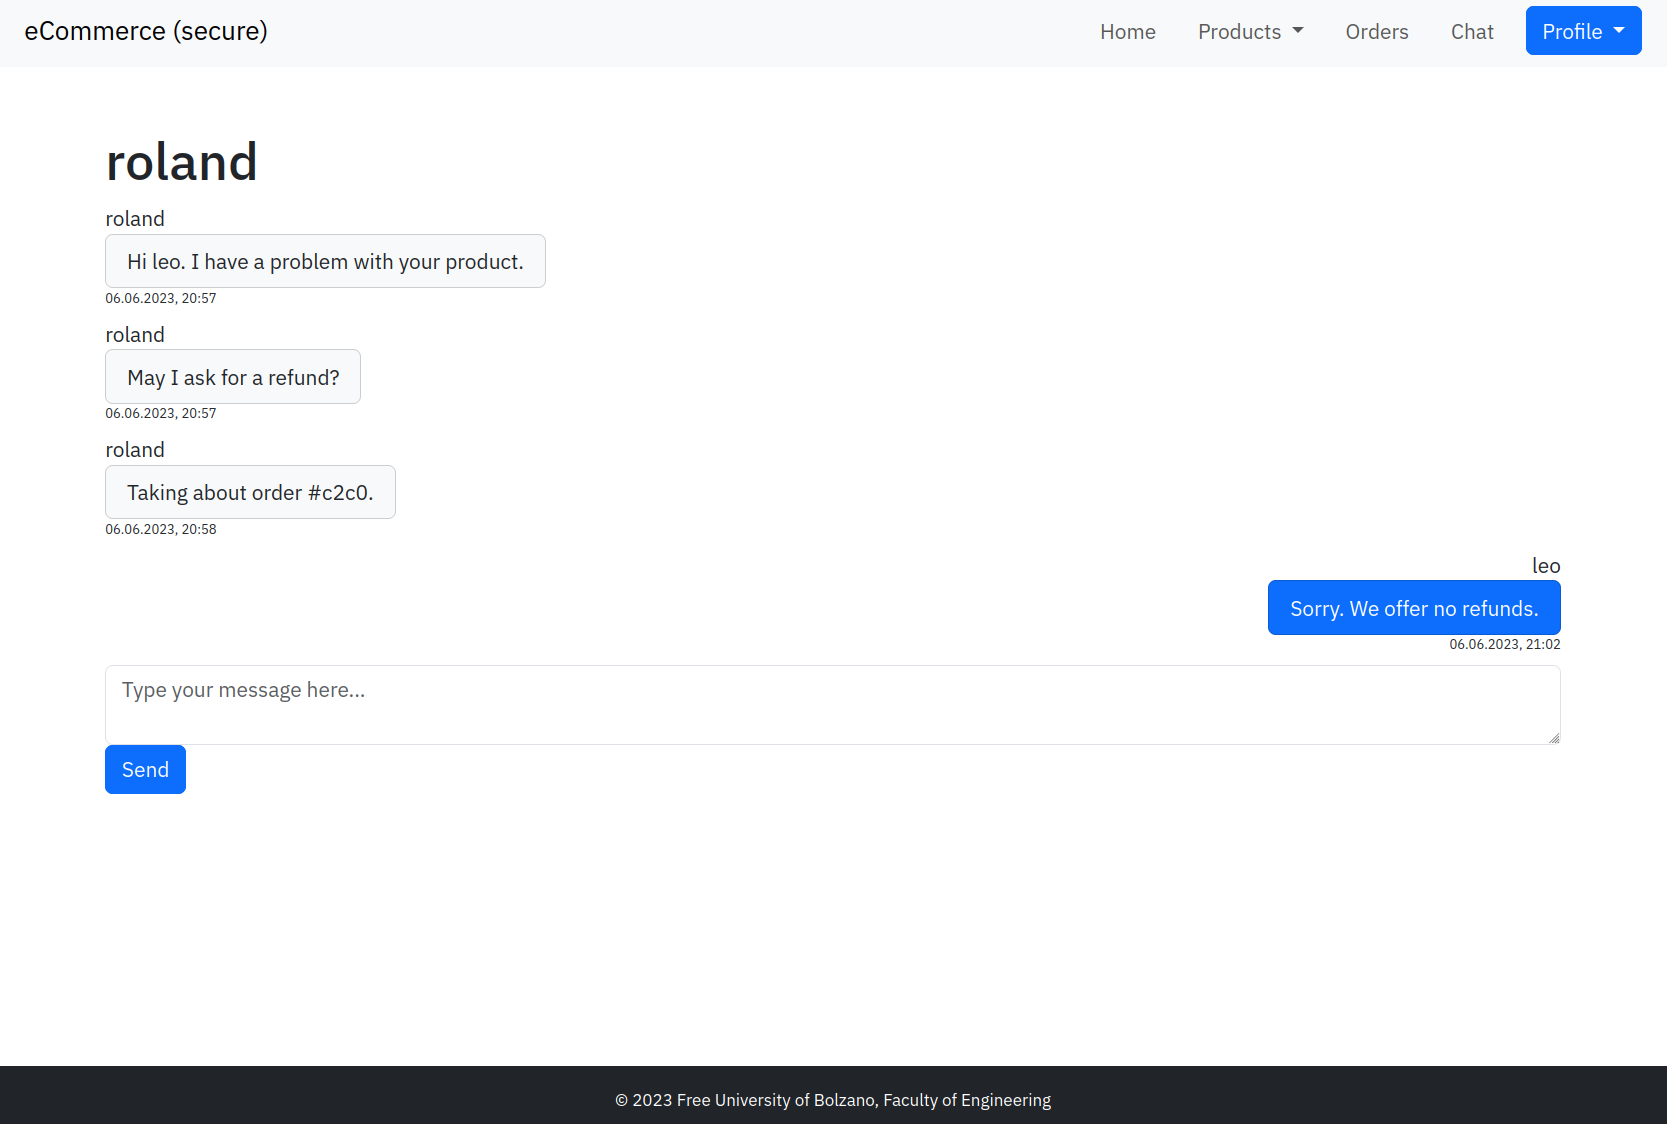
\includegraphics[width=\linewidth]{resources/chat.png}
        \caption{An example chat between vendor and customer.}
    \end{subfigure}
    \caption{Example showing how customers can chat with vendors.}
\end{figure}

The application offers the customers the ability to message vendors over a private chat. The customers can click on the name of the vendor beneath the product name on the product information page. This will bring them to the direct chat page for the selected vendor. All chats the customer has started are also available in the chats list by navigating using the “Chats” button in the header of the webpage. By selecting one of the chats, the user is able to type a message into the text area at the bottom of the page and click “Send” to send me message. Messages are stored encrypted using the DES algorithm and are not accessible to anyone but the users participating in the communication.


\end{document}
